% Options for packages loaded elsewhere
\PassOptionsToPackage{unicode}{hyperref}
\PassOptionsToPackage{hyphens}{url}
%
\documentclass[
]{article}
\usepackage{amsmath,amssymb}
\usepackage{iftex}
\ifPDFTeX
  \usepackage[T1]{fontenc}
  \usepackage[utf8]{inputenc}
  \usepackage{textcomp} % provide euro and other symbols
\else % if luatex or xetex
  \usepackage{unicode-math} % this also loads fontspec
  \defaultfontfeatures{Scale=MatchLowercase}
  \defaultfontfeatures[\rmfamily]{Ligatures=TeX,Scale=1}
\fi
\usepackage{lmodern}
\ifPDFTeX\else
  % xetex/luatex font selection
\fi
% Use upquote if available, for straight quotes in verbatim environments
\IfFileExists{upquote.sty}{\usepackage{upquote}}{}
\IfFileExists{microtype.sty}{% use microtype if available
  \usepackage[]{microtype}
  \UseMicrotypeSet[protrusion]{basicmath} % disable protrusion for tt fonts
}{}
\makeatletter
\@ifundefined{KOMAClassName}{% if non-KOMA class
  \IfFileExists{parskip.sty}{%
    \usepackage{parskip}
  }{% else
    \setlength{\parindent}{0pt}
    \setlength{\parskip}{6pt plus 2pt minus 1pt}}
}{% if KOMA class
  \KOMAoptions{parskip=half}}
\makeatother
\usepackage{xcolor}
\usepackage[margin=1in]{geometry}
\usepackage{color}
\usepackage{fancyvrb}
\newcommand{\VerbBar}{|}
\newcommand{\VERB}{\Verb[commandchars=\\\{\}]}
\DefineVerbatimEnvironment{Highlighting}{Verbatim}{commandchars=\\\{\}}
% Add ',fontsize=\small' for more characters per line
\usepackage{framed}
\definecolor{shadecolor}{RGB}{248,248,248}
\newenvironment{Shaded}{\begin{snugshade}}{\end{snugshade}}
\newcommand{\AlertTok}[1]{\textcolor[rgb]{0.94,0.16,0.16}{#1}}
\newcommand{\AnnotationTok}[1]{\textcolor[rgb]{0.56,0.35,0.01}{\textbf{\textit{#1}}}}
\newcommand{\AttributeTok}[1]{\textcolor[rgb]{0.13,0.29,0.53}{#1}}
\newcommand{\BaseNTok}[1]{\textcolor[rgb]{0.00,0.00,0.81}{#1}}
\newcommand{\BuiltInTok}[1]{#1}
\newcommand{\CharTok}[1]{\textcolor[rgb]{0.31,0.60,0.02}{#1}}
\newcommand{\CommentTok}[1]{\textcolor[rgb]{0.56,0.35,0.01}{\textit{#1}}}
\newcommand{\CommentVarTok}[1]{\textcolor[rgb]{0.56,0.35,0.01}{\textbf{\textit{#1}}}}
\newcommand{\ConstantTok}[1]{\textcolor[rgb]{0.56,0.35,0.01}{#1}}
\newcommand{\ControlFlowTok}[1]{\textcolor[rgb]{0.13,0.29,0.53}{\textbf{#1}}}
\newcommand{\DataTypeTok}[1]{\textcolor[rgb]{0.13,0.29,0.53}{#1}}
\newcommand{\DecValTok}[1]{\textcolor[rgb]{0.00,0.00,0.81}{#1}}
\newcommand{\DocumentationTok}[1]{\textcolor[rgb]{0.56,0.35,0.01}{\textbf{\textit{#1}}}}
\newcommand{\ErrorTok}[1]{\textcolor[rgb]{0.64,0.00,0.00}{\textbf{#1}}}
\newcommand{\ExtensionTok}[1]{#1}
\newcommand{\FloatTok}[1]{\textcolor[rgb]{0.00,0.00,0.81}{#1}}
\newcommand{\FunctionTok}[1]{\textcolor[rgb]{0.13,0.29,0.53}{\textbf{#1}}}
\newcommand{\ImportTok}[1]{#1}
\newcommand{\InformationTok}[1]{\textcolor[rgb]{0.56,0.35,0.01}{\textbf{\textit{#1}}}}
\newcommand{\KeywordTok}[1]{\textcolor[rgb]{0.13,0.29,0.53}{\textbf{#1}}}
\newcommand{\NormalTok}[1]{#1}
\newcommand{\OperatorTok}[1]{\textcolor[rgb]{0.81,0.36,0.00}{\textbf{#1}}}
\newcommand{\OtherTok}[1]{\textcolor[rgb]{0.56,0.35,0.01}{#1}}
\newcommand{\PreprocessorTok}[1]{\textcolor[rgb]{0.56,0.35,0.01}{\textit{#1}}}
\newcommand{\RegionMarkerTok}[1]{#1}
\newcommand{\SpecialCharTok}[1]{\textcolor[rgb]{0.81,0.36,0.00}{\textbf{#1}}}
\newcommand{\SpecialStringTok}[1]{\textcolor[rgb]{0.31,0.60,0.02}{#1}}
\newcommand{\StringTok}[1]{\textcolor[rgb]{0.31,0.60,0.02}{#1}}
\newcommand{\VariableTok}[1]{\textcolor[rgb]{0.00,0.00,0.00}{#1}}
\newcommand{\VerbatimStringTok}[1]{\textcolor[rgb]{0.31,0.60,0.02}{#1}}
\newcommand{\WarningTok}[1]{\textcolor[rgb]{0.56,0.35,0.01}{\textbf{\textit{#1}}}}
\usepackage{longtable,booktabs,array}
\usepackage{calc} % for calculating minipage widths
% Correct order of tables after \paragraph or \subparagraph
\usepackage{etoolbox}
\makeatletter
\patchcmd\longtable{\par}{\if@noskipsec\mbox{}\fi\par}{}{}
\makeatother
% Allow footnotes in longtable head/foot
\IfFileExists{footnotehyper.sty}{\usepackage{footnotehyper}}{\usepackage{footnote}}
\makesavenoteenv{longtable}
\usepackage{graphicx}
\makeatletter
\def\maxwidth{\ifdim\Gin@nat@width>\linewidth\linewidth\else\Gin@nat@width\fi}
\def\maxheight{\ifdim\Gin@nat@height>\textheight\textheight\else\Gin@nat@height\fi}
\makeatother
% Scale images if necessary, so that they will not overflow the page
% margins by default, and it is still possible to overwrite the defaults
% using explicit options in \includegraphics[width, height, ...]{}
\setkeys{Gin}{width=\maxwidth,height=\maxheight,keepaspectratio}
% Set default figure placement to htbp
\makeatletter
\def\fps@figure{htbp}
\makeatother
\setlength{\emergencystretch}{3em} % prevent overfull lines
\providecommand{\tightlist}{%
  \setlength{\itemsep}{0pt}\setlength{\parskip}{0pt}}
\setcounter{secnumdepth}{-\maxdimen} % remove section numbering
\ifLuaTeX
  \usepackage{selnolig}  % disable illegal ligatures
\fi
\usepackage{bookmark}
\IfFileExists{xurl.sty}{\usepackage{xurl}}{} % add URL line breaks if available
\urlstyle{same}
\hypersetup{
  pdftitle={HW X},
  pdfauthor={Andrew Jowe},
  hidelinks,
  pdfcreator={LaTeX via pandoc}}

\title{HW X}
\author{Andrew Jowe}
\date{}

\begin{document}
\maketitle

\section{I Introduction}\label{i-introduction}

Question: How does the annual salary (USD) vary between different
professions (Data Scientist, Software Engineer, Bioinformatics Engineer)
across different regions (San Francisco and Seattle)?

Interest: Understanding the salary distribution across professions and
regions can provide insightful economic. Insights into wage can help
individuals make informed decisions about career paths and relocation
opportunities. Additionally, businesses and governments can use this
information to strategize their hiring plans and economic policies
respectively.

Approach: Two Factor ANOVA (TFA)

\section{II. Summary}\label{ii.-summary}

It is important to understand and summarize the data to conduct an
insightful analysis of the relationship between annual salaries among
different professions and regions. By interpreting the sampled annual
salary data, we can examine important measurements through statistical
tables, and visualize the distribution of the data through plots.
Overall allowing the discovery of trends that can not be seen just by
looking at data alone.

In this section, we will summarize the randomly sampled and observed
annual salary data according to its general distribution, distribution
by category, and distribution among categories.

\subsection{II-1 Overall Distribution of Sample
Data}\label{ii-1-overall-distribution-of-sample-data}

Looking at the overall distribution of the Annual salary sample data
allows us to grasp a general trend of the data distribution.

To interpret the numerical values (Annual Salary), the data can be
plotted into a histogram to visualize the variability of the overall
sample population (Figure 2.1).

\textbf{Figure 2.1}

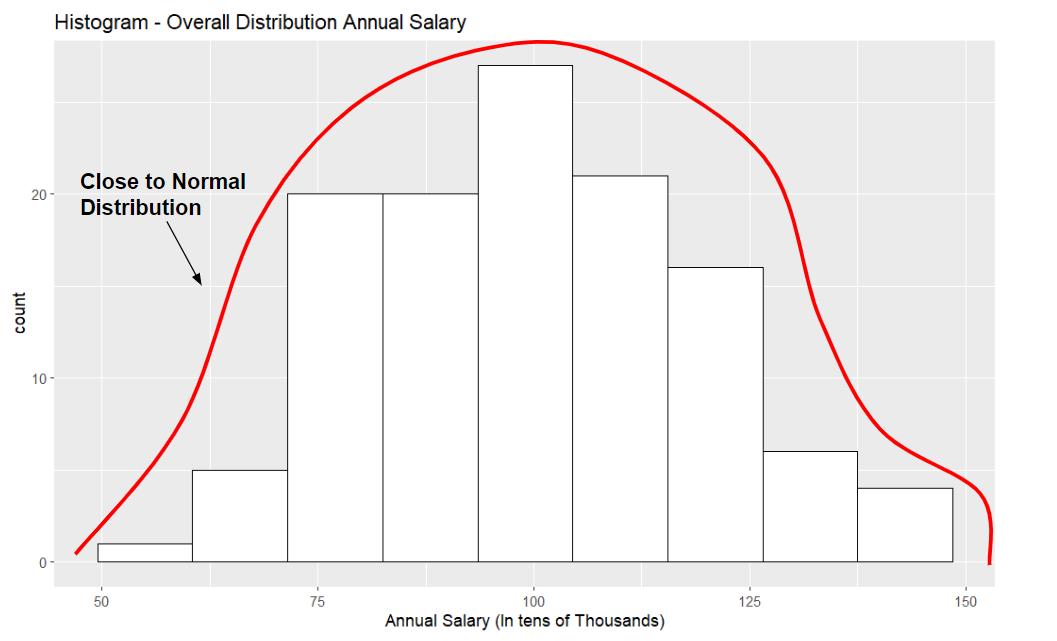
\includegraphics[width=7.29167in,height=\textheight]{Overall data Histogram.png}

Figure 2.1 sorts the overall sample population (120 data points) by the
frequency of the annual salary according to a range. Each bar has a bin
size of 11, meaning that each bar represents a range of \$11,000. Hence,
the y-axis represents the frequency of a salary every \$11,000. The
highest frequency (the mode) of around 27 people tends to occur around
the range of around \$94,000-105,000, which also consists of the mean.
The lowest frequency of around 1 person occurs at the smallest salary of
around \$50,000-\$61,000. These values, along with the general symmetry
of the data above allow us to assume that the distribution of Salary is
almost normal, with a slight left tail. This could mean that the average
person for all professions and regions in our sample tends to earn a bit
more than \$100,000.

While a Histogram gives us a general visualization of the salary
distribution, it does not do well to give a more accurate representation
of the symmetry if there are outlier's.

Analysis of the overall distribution of salary through a box plot helps
clarify the symmetry of the data as it omits the outlier's and sees the
spread of the data majority.

\textbf{Figure 2.2}

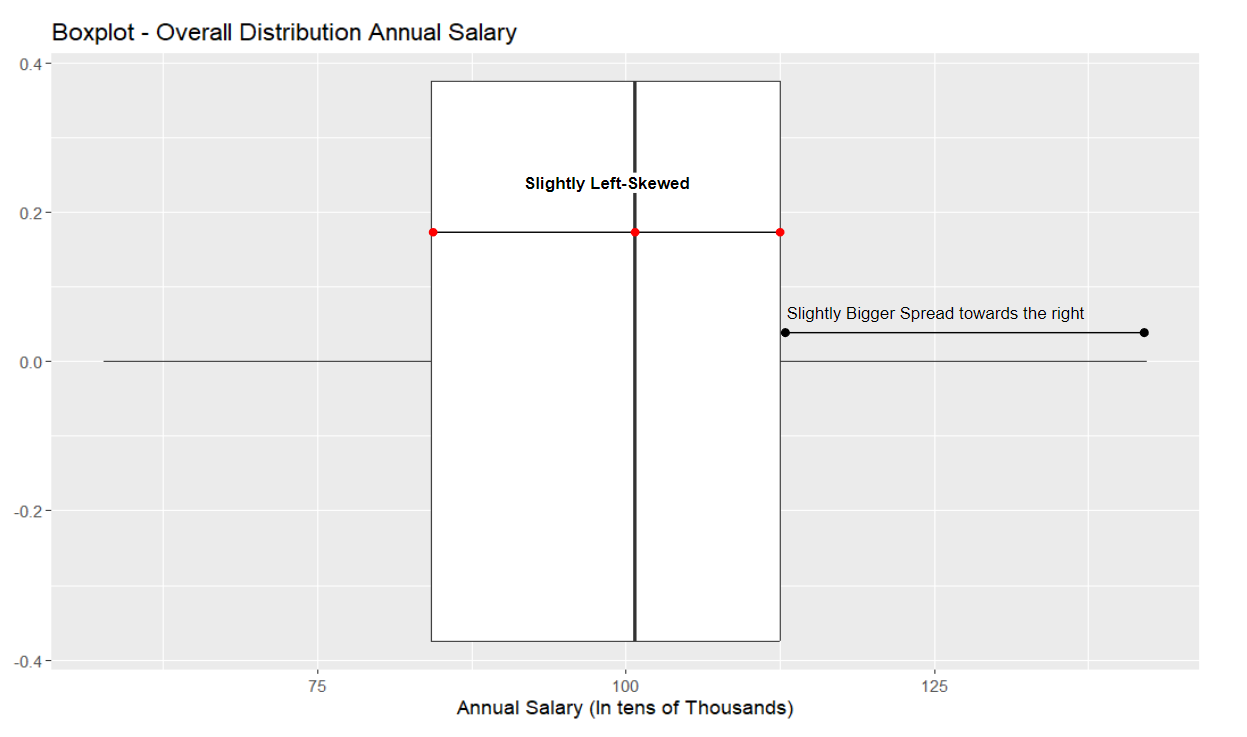
\includegraphics[width=7.29167in,height=\textheight]{Overall Data Boxplot.png}

Figure 2.2 shows that the sample population does not consist of any
outlier's (numerically distant points). Giving a further indication of
its relatively normal distribution. The lower 25\% whisker of
\textasciitilde\$60-84 thousand is smaller than the upper 25\% whisker
of around \$112.5-140 thousand, giving evidence of a slight left tail.
The middle 50\% (Interquartile range) has a slight left skew where the
median is bigger than the mean. However, the interquartile range stays
relatively in the middle. Meaning that the data has a relatively normal
distribution.

In summary, through a general analysis of the annual salaries without
taking different categories into account, it can be concluded that the
data has an almost normal distribution with no outlier's and a slight
bias towards the right (higher salary).

\subsection{II-2 Distribution of Annual Salary by
Category}\label{ii-2-distribution-of-annual-salary-by-category}

While the data above gave us a general idea of the distribution of the
data, it does not tell us the distribution of data within each group.
Conducting further observations of the data distribution according to
each group per category allows us to analyze how each category has an
impact on salary distribution.

The Salary Data Set is Distributed into 2 categories:

\begin{itemize}
\item
  \textbf{Profession:} With groups DS (Data-Scientist), SE
  (Software-Engineer), BE (Bioinformatics Engineer)
\item
  \textbf{Region:} With groups SF (San Francisco), S (Seattle)
\end{itemize}

\textbf{Figure 2.3}

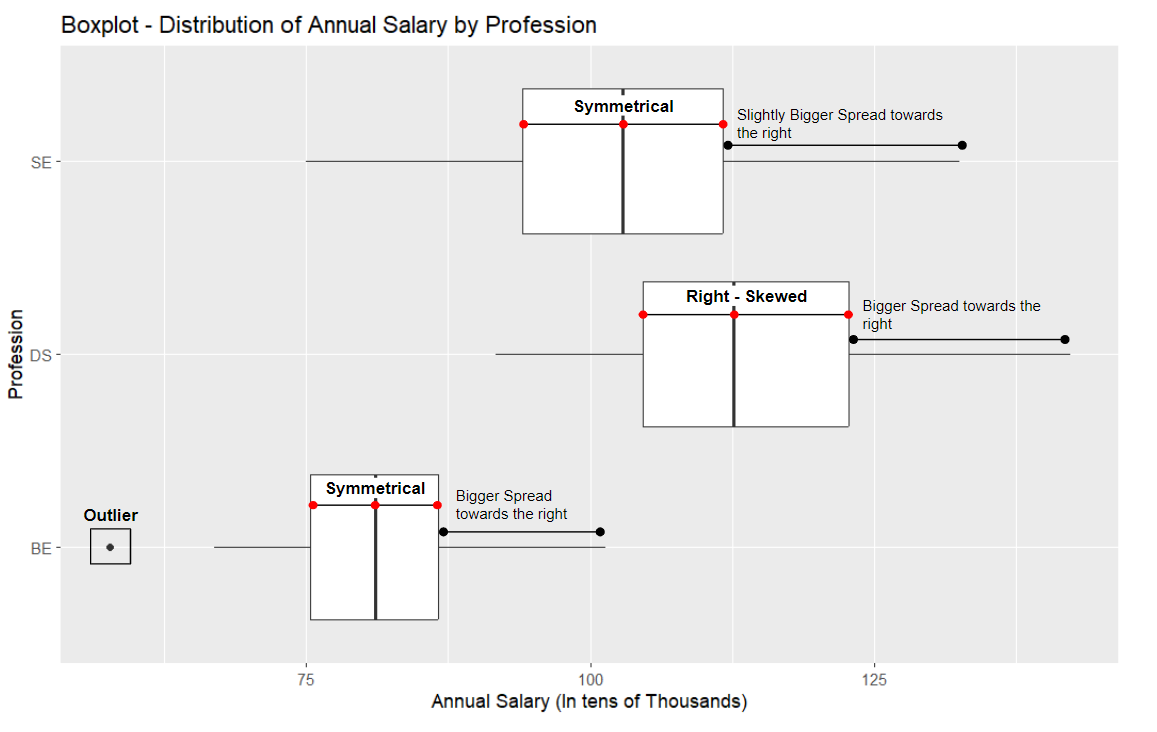
\includegraphics[width=7.29167in,height=\textheight]{Profession Data Boxplot.png}

Figure 2.3 structures the Annual Salary of each worker by their
profession. Based on the medians of each profession, Bioinformatics
Engineers tend to earn the lowest and Data Scientists tend to earn the
highest. The interquartile range further suggest the approximate
normality of the data. However, it can be noted that majority of
Data-Scientists tend to earn more than the median, and that one
bioinformatic engineer tends to earn a lower salary than the sampled
data of bioinformatic engineers. However, these points will not majorly
affect our data.

The highest variability in salary occurs among Data Scientists and
Bioinformatics engineers, in which the right tailed-bias (smaller
left-whisker and bigger right-whisker) along with the symmetry in IQR
suggests that the average salary per worker (mean) is higher than the
median.

\textbf{Figure 2.4}

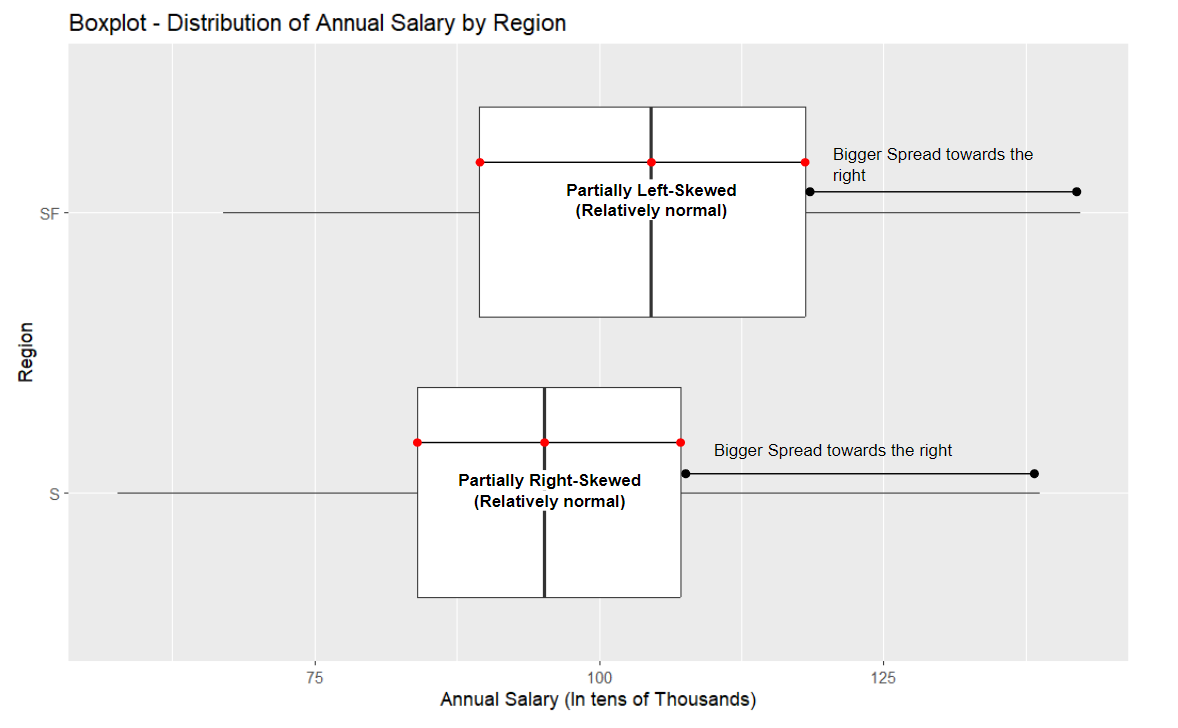
\includegraphics[width=7.29167in,height=\textheight]{Region Data Boxplot.png}

Figure 2.4 structures the annual salary per worker by the region they
are in. While the median salary for workers in San Francisco appears to
be higher than workers in Seattle, they are not beyond the bounds of the
other regions IQR. Suggesting that it may be an insignificant
difference. Therefore the interquartile range may further suggest the
approximate normality of the data, which we will analyze further in the
analysis section.

\subsection{II-3 Mean distribution of Annual Salary among
categories}\label{ii-3-mean-distribution-of-annual-salary-among-categories}

\subsubsection{II-3.1 Analysis of sample
means}\label{ii-3.1-analysis-of-sample-means}

To further understand the interaction between the numerical values
(annual salary), and the categorical values (Profession and Region), a
interaction plot and a summary of mean values can be looked at.

To simplify the interpretation, the categories will be referred to as
Factors.

\begin{itemize}
\item
  \textbf{Factor A:} Profession, with values Data Scientist (DS),
  Software Engineer (SE), and Bioinformatics Engineer (BE)
\item
  \textbf{Factor B:} Region, with values San Francisco (SF) and Seattle
  (S)
\end{itemize}

\textbf{Figure 2.5}

\begin{longtable}[]{@{}
  >{\raggedright\arraybackslash}p{(\columnwidth - 8\tabcolsep) * \real{0.2500}}
  >{\raggedright\arraybackslash}p{(\columnwidth - 8\tabcolsep) * \real{0.1765}}
  >{\raggedright\arraybackslash}p{(\columnwidth - 8\tabcolsep) * \real{0.1912}}
  >{\raggedright\arraybackslash}p{(\columnwidth - 8\tabcolsep) * \real{0.1912}}
  >{\raggedright\arraybackslash}p{(\columnwidth - 8\tabcolsep) * \real{0.1912}}@{}}
\toprule\noalign{}
\begin{minipage}[b]{\linewidth}\raggedright
\end{minipage} & \begin{minipage}[b]{\linewidth}\raggedright
BE
\end{minipage} & \begin{minipage}[b]{\linewidth}\raggedright
DS
\end{minipage} & \begin{minipage}[b]{\linewidth}\raggedright
SE
\end{minipage} & \begin{minipage}[b]{\linewidth}\raggedright
Group Means
\end{minipage} \\
\midrule\noalign{}
\endhead
\bottomrule\noalign{}
\endlastfoot
\textbf{S} & 79.75 (20) & 112.53 (20) & 95.55 (20) & 95.94 (60) \\
\textbf{SF} & 82.42(20) & 117.77 (20) & 110.26 (20) & 103.48 (60) \\
\textbf{Group Means} & 81.09(40) & 115.15 (40) & 102.91 (40) & 99.71
(120) \\
\end{longtable}

Figure 2.5 sorts each factor (A,B) by their average mean salary, and the
value in parentheses shows the sample size of each interaction. Data
Scientists in San Francisco tend to have the highest salary while
Bioinformatics Engineers in Seattle tend to have the lowest. As all
sample sizes are equal, it eliminates the possibility of a weightage
bias in the overall factor mean.

When comparing the factor means to the overall sample mean, we can see
that there is a bigger difference in worker salary when it comes to
profession more than region. The difference ranges from \$3.2-18.62
thousand according to profession and ±\$3.77 thousand according to
region.

Comparing pairwise differences of the individual Factor B (region)
samples to the overall Factor B mean, we can see that there is not a
significant difference in average salary for Bioinformatic Engineers and
Data Scientists in a given region. With a difference ranging from
\$1.33-1.34 thousand for Bioinformatic Engineers, and ±\$2.62 thousand
for DS. However, software engineers have a \$7.35-7.36 thousand
difference in Salary depending on what region they work in. Meaning that
Factor B may not have a major impact on salary except for Software
Engineers. As for comparing individual means of factor A (Profession) to
the overall mean of factor A, we can see that there is a significant
difference in average salary depending on the profession. With a range
of \$0.39-16.59 thousand for workers in Seattle, and \$6.78-21.06
thousand for workers in San Francisco. This gives evidence of a possible
interaction effect, with factor A having a stronger impact than factor
B. However, further analysis testing through formal models is needed to
conclude an interaction.

While the summary of mean values gives a numerical perspective of the
sample salary distribution among workers according to profession and
region, looking at the factors through an interaction plot is an
informal method to gain a visual perspective on how profession and
region interact to effect the average annual salary of a worker. It
could also give further evidence of a possible interaction effect
between both factors.

\textbf{Figure 2.6}

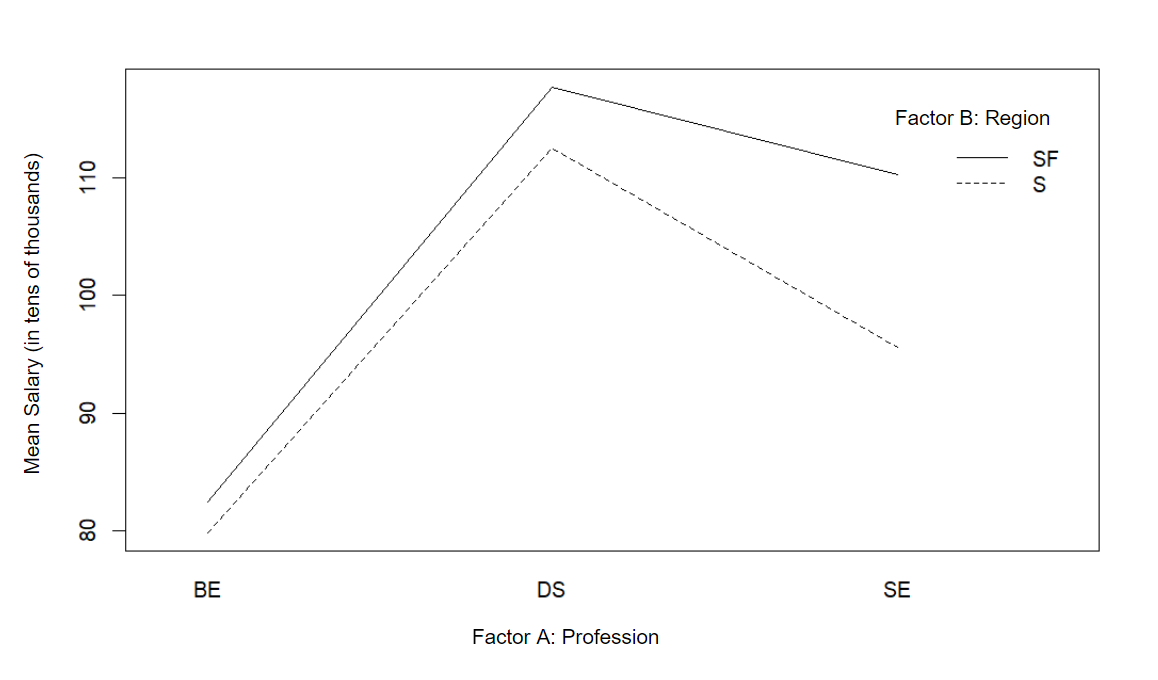
\includegraphics[width=7.29167in,height=\textheight]{Interaction Plot.png}

As seeen in Figure 2.6, the interaction plot further suggests a possible
interaction effect between Profession and region. This can be seen as
the slopes of SF and S do not run parallel to each other from BE to DS
and DS to SE. Additionally, the steeper (bigger) slope between DS and SE
in Seattle compared to San Francisco suggests that the difference in pay
between data scientists and software engineers is a lot larger in
Seattle than San Francisco, possibly meaning an interaction.

Comparing pairwise differences, it it seen that there is a larger
difference in salaries (income gap) for software engineers in both
regions as compared to the other 2 professions. This observation could
mean that there is a higher demand for Software engineers in San
Francisco than in Seattle, and that there is an interaction effect which
we can further analyze in our analysis.

\subsubsection{II-3.2 Analysis of group
variances}\label{ii-3.2-analysis-of-group-variances}

\textbf{Figure 2.7}

\textbf{Overall (Sample) Standard Deviation -} 18.70

\begin{longtable}[]{@{}llll@{}}
\toprule\noalign{}
\textbf{Profession} & \textbf{BE} & \textbf{DS} & \textbf{SE} \\
\midrule\noalign{}
\endhead
\bottomrule\noalign{}
\endlastfoot
Standard Deviation & 9.67 & 13.67 & 13.24 \\
\textbf{Region} & \textbf{S} & \textbf{SF} & \\
Standard Deviation & 17.42 & 19.30 & \\
\end{longtable}

An analysis of group standard deviations allows us to understand the
spread of each group from its group mean. Where a lower spread (standard
deviation) indicates the group values are denser near the mean. Overall,
the salaries by group tend to vary from \$9.67-\$19.30 thousand per
worker, which is around 10\%-19\% of the overall average salary per
worker.

Through a comparison of the group standard deviations from the overall
standard deviation, we can see that the standard deviation's for every
group in the profession category is much lesser than the overall
standard deviation compared to region. With a difference of 5.03-5.46
for profession and 0.6-1.28 for region from the overall standard
deviation.

The standard deviation further allows us to interpret the difference in
means. Since the average salary of a data scientist is more than 3
standard deviations (around 3.52) away from a Bioinformatics Engineer
average salary, it suggests a difference in average salary between data
scientists and bioinformatics engineers as the spread is high. In the
same manner, the average salary of a worker in San Francisco is less
than 1 standard deviation (around 0.43) away from the average salary of
a worker in Seattle, suggesting a possibility of a lower difference is
sample means.

In general, the difference in standard deviations among groups suggest
that the sample have a roughly constant variance within each category.
With a range of \$0.43-4 thousand among profession and \$1.88 thousand
among region. Further diagnostic testing will be conducted to verify
this.

\subsection{II-4 Summary}\label{ii-4-summary}

In summary, the relatively normal distribution of normal salary and the
relatively constant standard deviation suggests that our ANOVA
assumptions are met. Through an analysis of the factor means, it appears
that the profession (factor A) of the worker has a stronger individual
impact on annual salary than the region (factor B) the worker is in.
Even so, there appears to be an interaction effect between both factors
on annual salary, where profession affects the salary of all regions and
region impacts the salary of Software Engineers but not any other
profession.

What could this mean.

While this section gave a relative understanding of the distribution of
Annual salary per category, an analysis through formal models and
methods is required to make a more accurate conclusion.

\section{III Diagnostics}\label{iii-diagnostics}

In this section, we will check whether our data satisfies the ANOVA
assumptions.

The assumptions are: 1. All samples are independent 2. All groups in
factor \(A\) are independent 3. All groups in factor \(B\) are
independent 4. Errors are normally distributed and have constant
variance where \(\epsilon_{ij} \sim N(0, \sigma_\epsilon^2)\)

Due to limitations, we can only test whether the errors are normally
distributed and have constant variance. We cannot determine whether
assumptions one through three are satisfied as we did not sample the
data. For simplicity, we will assume these hold.

\subsection{III.1 Assessing Type I and Type II
Errors}\label{iii.1-assessing-type-i-and-type-ii-errors}

To determine which \(\alpha\) to use for diagnostics, we need to assess
whether we want to minimize the chance of a Type I Error or a Type II
Error.

\begin{itemize}
\tightlist
\item
  Type I Error: When you reject \(H_0\) when in reality \(H_0\) is true.
  In this case, this represents the chance we conclude the data violates
  our ANOVA assumptions when in reality it satisfies our ANOVA
  assumptions.
\item
  Type II Error: When you accept \(H_0\) when in reality \(H_0\) is
  false. In this case, this represents the chance we conclude the data
  satisfies our ANOVA assumptions when in reality it violates our ANOVA
  assumptions
\end{itemize}

For determining normality and constant variance, we want to minimize our
probability of incorrect assumptions, so a Type II error is worse than a
Type I error. As a result, we want to maximize \(\alpha\), so we will
use \(\alpha = 0.1\) as our threshold.

\subsection{III.2 Determine Normality}\label{iii.2-determine-normality}

\subsubsection{III.2.1 QQ Plot}\label{iii.2.1-qq-plot}

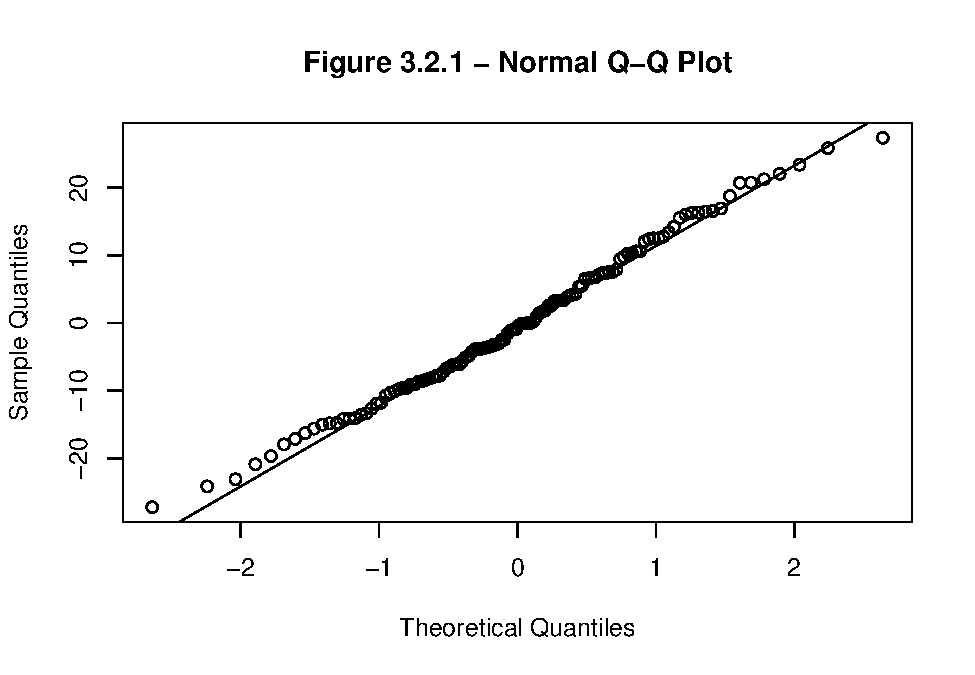
\includegraphics{STA_106_Project_2_files/figure-latex/unnamed-chunk-4-1.pdf}

The QQ plot shows our original data plotted against a theoretical normal
distribution. From the plot, the majority of the data points converge to
the normal line, suggesting that our data is most likely normal. We
formalize this plot by running a Shapiro-Wilk Test next.

\subsubsection{III.2.2 Shapiro Wilk
Test}\label{iii.2.2-shapiro-wilk-test}

\(H_0:\) Our data is normal.

\(H_a:\) Our data is not normal.

\(p = 0.6698\)

Since \(p > \alpha\), we accept \(H_0\). Therefore, our data is normal.

\subsection{III.3 Assessing Constant
Variance}\label{iii.3-assessing-constant-variance}

\subsubsection{III.3.1 Plot on Errors vs Groups
Means}\label{iii.3.1-plot-on-errors-vs-groups-means}

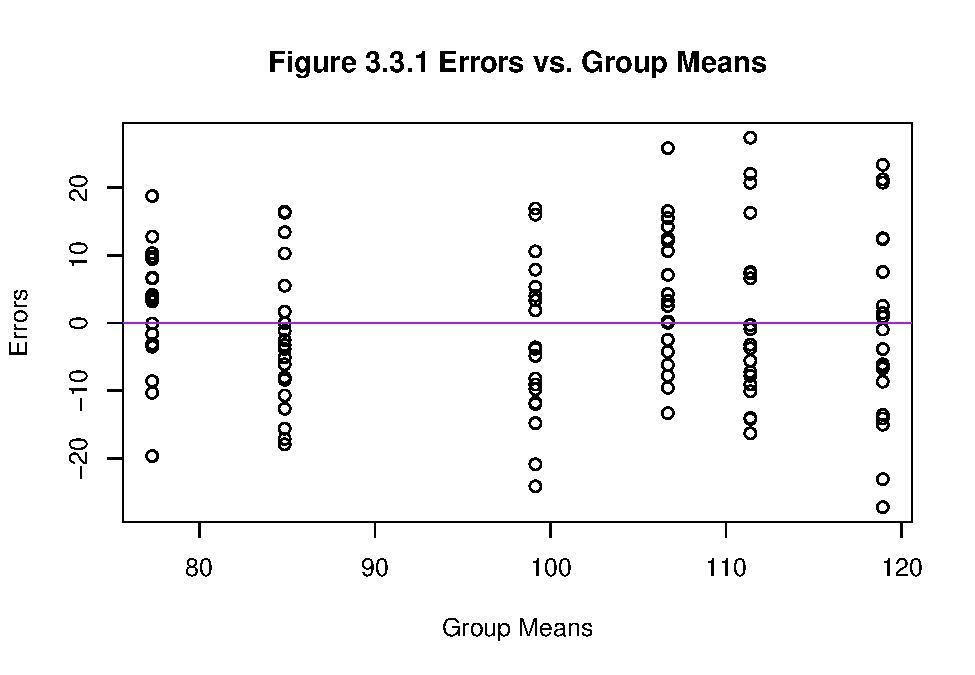
\includegraphics{STA_106_Project_2_files/figure-latex/unnamed-chunk-6-1.pdf}

From figure 3.3.1, the dots for each group mean seem to have
approximately the same spread, suggesting that there is constant
variance between groups. To formalize this, we will run the BF-test
next.

\subsubsection{III.3.2 BF-Test}\label{iii.3.2-bf-test}

\begin{verbatim}
## Warning in leveneTest.default(y = y, group = group, ...): group coerced to
## factor.
\end{verbatim}

\(H_0:\) The data have constant variances.

\(H_a:\) The data does not have constant variances.

Since \(p = 0.3048 > \alpha\), we accept \(H_0\). Therefore, the data
has constant variances.

\subsection{III.4 Final Verdict}\label{iii.4-final-verdict}

We can conclude that the errors are normally distributed and have
constant variances, satisfying one of our ANOVA assumptions. No
transformation nor outlier removal is needed.

\section{IV Analysis and
Interpretation}\label{iv-analysis-and-interpretation}

\subsection{IV.1 Finding Best Model}\label{iv.1-finding-best-model}

We will first observe the conditional \(R^2\) and differences between
mean values to see what to expect. Then we will use F-statistic test to
find out which model to use. When conducting our test, we will first
test for interaction effect. If there is interaction effect, we use the
model with interaction effect and stop the testing. Otherwise, we will
continue testing for factor A and factor B. We will only use these
factors if there are significant effects.

\subsubsection{\texorpdfstring{IV.1.1 Conditional
\(R^2\)}{IV.1.1 Conditional R\^{}2}}\label{iv.1.1-conditional-r2}

\textbf{Figure 4.1.1}

\begin{longtable}[]{@{}lrrrrr@{}}
\toprule\noalign{}
& AB & X.A.B. & A & B & Empty.Null \\
\midrule\noalign{}
\endhead
\bottomrule\noalign{}
\endlastfoot
SSE & 15252.93 & 16058.34 & 17764.09 & 39872.94 & 41578.69 \\
\end{longtable}

\textbf{Figure 4.1.2}

\begin{longtable}[]{@{}
  >{\raggedleft\arraybackslash}p{(\columnwidth - 8\tabcolsep) * \real{0.2079}}
  >{\raggedleft\arraybackslash}p{(\columnwidth - 8\tabcolsep) * \real{0.1980}}
  >{\raggedleft\arraybackslash}p{(\columnwidth - 8\tabcolsep) * \real{0.1980}}
  >{\raggedleft\arraybackslash}p{(\columnwidth - 8\tabcolsep) * \real{0.1980}}
  >{\raggedleft\arraybackslash}p{(\columnwidth - 8\tabcolsep) * \real{0.1980}}@{}}
\toprule\noalign{}
\begin{minipage}[b]{\linewidth}\raggedleft
\(R^2(AB&#124;(A+B))\)
\end{minipage} & \begin{minipage}[b]{\linewidth}\raggedleft
\(R^2((A+B)&#124;A)\)
\end{minipage} & \begin{minipage}[b]{\linewidth}\raggedleft
\(R^2((A+B)&#124;B)\)
\end{minipage} & \begin{minipage}[b]{\linewidth}\raggedleft
\(R^2(A&#124;Empty)\)
\end{minipage} & \begin{minipage}[b]{\linewidth}\raggedleft
\(R^2(B&#124;Empty)\)
\end{minipage} \\
\midrule\noalign{}
\endhead
\bottomrule\noalign{}
\endlastfoot
0.0502 & 0.096 & 0.5973 & 0.5728 & 0.041 \\
\end{longtable}

From figure 4.1.2, there seems to be a significant factor A effect since
its \(R^2\) value is large when adding it both to the empty model and
the model with factor B. While the conditional \(R^2\) may hint which
factors may be significant, this is not a conclusive test.

\subsubsection{IV.1.2 Assessing Type I and Type II
Errors}\label{iv.1.2-assessing-type-i-and-type-ii-errors}

To determine which \(\alpha\) to use for diagnostics, we need to assess
whether we want to minimize the chance of a Type I Error or a Type II
Error.

Type I Error: The chance we reject \(H_0\) when in reality \(H_0\) is
true. In this case, it is the chance we conclude that there is a
significant effect when in reality there is no significant effect.

Type II Error: The chance that we accept \(H_0\) when in reality \(H_0\)
is false. In this case, it is the chance we conclude that there is no
significant effect when in reality there is a significant effect.

In our analysis, we want to capture the factor and interaction effects
if it exists, and thus want to minimize unexplained error. The lower the
Type II Error, the less chance of falsely concluding no significant
effect, increasing the chance of less unexplained error. Since a type II
error is worse, we want to minimize it, so we will choose a higher
\(\alpha\) value. As a result, we will choose \(\alpha = 0.1\).

\subsubsection{IV.1.3 Testing for Interaction
Effect}\label{iv.1.3-testing-for-interaction-effect}

Our full model is
\(Y_{ijk} = \mu_{ij} + \gamma_i + \delta_j + (\gamma\delta)_{ij} + \epsilon_{ijk}\)

With constraints: - \(\sum \gamma_i = 0\) - \(\sum \delta_j = 0\) -
\(\sum \sum (\gamma_i \delta_j) = 0\)

Our reduced model is
\(Y_{ijk} = \mu_{ij} + \gamma_i + \delta_j + \epsilon_{ijk}\)

With constraints: - \(\sum \gamma_i = 0\) - \(\sum \delta_j = 0\)

Hypothesis: - \(H_0:\) There is no significant interaction effect
(i.e.~all \((\gamma\delta)_{ij} = 0\)). Do not use the full model. -
\(H_a:\) There is significant interaction effect (i.e.~at least one
\((\gamma\delta)_{ij} \neq 0\)). Use the full model.

Test results: - \(F_s = 3.0098\) - \(p = 0.0532\)

Since \(p \leq \alpha\), we reject \(H_0\). Therefore, we will use the
full model.

\subsubsection{IV.1.4 Model Choice}\label{iv.1.4-model-choice}

From our testing, our final model choice is
\(Y_{ijk} = \mu_{ij} + \gamma_i + \delta_j + (\gamma \delta)_{ij} + \epsilon{ijk}\)

With constraints: - \(\sum \gamma_i = 0\) - \(\sum \delta_j = 0\) -
\(\sum \sum (\gamma_i \delta_j) = 0\)

\subsection{IV.2 Comparisons of Different
Factors}\label{iv.2-comparisons-of-different-factors}

First, we will create pairwise confidence intervals to test how much
professions affects average annual salary. Then, we will create another
pairwise interval to test how much region affects average annual salary.
Lastly, we will create non-pairwise intervals to test for more complex
differences.

\subsubsection{IV.2.1 Accuracy}\label{iv.2.1-accuracy}

We want to minimize the error of our confidence interval for stronger
interpretation. As a result, we want to minimize the probability that
the value does not lie within our confidence interval by minimizing
\(\alpha\). Therefore, we will choose \(\alpha = 0.001\).

\subsubsection{IV.2.2 Multiplier}\label{iv.2.2-multiplier}

We will compute 3 pairwise confidence intervals for group A and 1
pairwise confidence interval for group B to determine the difference in
annual salary given the difference in profession or region. For these
intervals, we can use either the Bonferonni, Tukey, or Scheffe
multipliers. We will pick the smallest multiplier for higher precision.

We will also compute 2 non-pairwise confidence intervals. For these
intervals, we cannot use Tukey since that is for pairwise comparisons
only. We will pick either Bonferonni or Scheffe, whichever one is
smaller.

\subsubsection{IV.2.3 Effect of Profession on Average Annual
Salary}\label{iv.2.3-effect-of-profession-on-average-annual-salary}

We will analyze the difference in average annual salary between all
professions.

Our 99.9\% confidence interval for the difference of average annual
salary between BE (bioinformatics engineer) and DS (data scientist) is
\([-43.6051, -24.5169]\). This means that we are 99.9\% confident that
on average BE makes around 24.5169 to 43.6051 less annually compared to
DS. Since 0 is not in our confidence interval, we are 99.9\% certain
that there is a difference in average annual salary between BE and DS
(i.e.~BS makes less than DS).

Our 99.9\% confidence interval for the difference of average annual
salary between DS and SE (software engineer) is \([2.6974, 21.7856]\).
This means that we are 99.9\% confident that on average DS makes around
2.6974 and 21.7856 more annually compared to SE. Since 0 is not in our
confidence interval, we are 99.9\% certain that there is a difference in
average annual salary between DS and SE (i.e.~DS makes more than SE).

Our 99.9\% confidence interval for the average difference of annual
salary between BE and SE is \([-31.3635, -12.2753]\). This means that we
are 99.9\% confident that on average BE makes around 12.2753 and 31.3635
less annually compared to SE. Since 0 is not in our confidence interval,
we are 99.9\% certain that there is a difference in average annual
salary between BE and SE (i.e.~BE makes more than SE).

\subsubsection{IV.2.4 Effect of Region on Average Annual
Salary}\label{iv.2.4-effect-of-region-on-average-annual-salary}

We will analyze the difference of average annual salary between S and
SF.

Our 99.9\% confidence interval for the average difference of annual
salary between S and SF is \([-14.6743, -0.4066]\). This means that we
are 99.9\% confident that on average people in S makes around 0.4066 and
14.6743 less annually compared to SF. Since 0 is not in our confidence
interval, we are 99.9\% certain that there is a difference in average
annual salary between people in S and SF (i.e.~S makes less than SF).

\subsubsection{IV.2.5 Addressing Large Salary Difference Between Regions
for
SE}\label{iv.2.5-addressing-large-salary-difference-between-regions-for-se}

From the summary, we see there is an interaction effect where SE gets
much higher pay in SF than S compared to other professions. This means
that regional differences may not apply to professions other than SE. We
will use pairwise confidence interval where we compare the effect of
different regions on average annual salary for average professional
other than SE.

Our 99.9\% confidence interval for the average difference in annual
salary between S and SF is \([-12.6901, 4.7841]\) for the average
professional other than SE. Since 0 is in our confidence interval, we
cannot conclude that there is a difference between regions for the
average professional other than SE. Therefore we believe that the result
from IV.2.4, the difference of average annual salary on region, mainly
applies to SE.

\subsubsection{IV.2.6 Addressing Wage Inequality in
SF}\label{iv.2.6-addressing-wage-inequality-in-sf}

From the summary, we noticed a huge gap between the average annual
salary for the lowest paying profession compared to the other
professions. This gap may be a sign of wage inequality. Lets test how
big this gap is.

Our 99.9\% confidence interval for the difference in average annual
salary between BE and the average profession other than BE is
\([-42.2981, -20.8966]\) for SF. This means that we are 99.9\% confident
that in SF the profession BE pays an average annual salary of around
20.8966 to 42.2981 lower than the average other professions. Since 0 is
not in our confidence interval, we conclude that there is a difference
between BE and the average other professions in SF.

\section{V Conclusion}\label{v-conclusion}

In conclusion, we find that the profession does affect annual salary. We
also found that region only affects salary for SE (software engineers).
Lastly, we found a significant wage gap between the lowest paying job,
BE (bioinfograhics enginering), and other professions in SF. We are
confident in our results as our data does not violate normality or
constant variance ANOVA assumptions, and in our diagnostics and we chose
conservative \(\alpha\) values for each test yielding more accurate
results.

One limitation is the fact that we have very few groups and not enough
data. For example, there are other technology roles like Machine
Learning and hardware engineering. We could have also separated entry
level roles from senior level roles. These ideas can present more
insighful results.

\newpage

\section{Appendix}\label{appendix}

\begin{Shaded}
\begin{Highlighting}[]
\CommentTok{\# Read the data from the downloaded file}
\NormalTok{file\_name }\OtherTok{\textless{}{-}} \StringTok{"Salary.csv"}
\NormalTok{data }\OtherTok{\textless{}{-}} \FunctionTok{read.csv}\NormalTok{(file\_name)}
\end{Highlighting}
\end{Shaded}

\begin{Shaded}
\begin{Highlighting}[]
\CommentTok{\# Give me means}
\NormalTok{find.means }\OtherTok{=} \ControlFlowTok{function}\NormalTok{(the.data,}\AttributeTok{fun.name =}\NormalTok{ mean)\{}
\NormalTok{  a }\OtherTok{=} \FunctionTok{length}\NormalTok{(}\FunctionTok{unique}\NormalTok{(the.data[,}\DecValTok{2}\NormalTok{]))}
\NormalTok{  b }\OtherTok{=} \FunctionTok{length}\NormalTok{(}\FunctionTok{unique}\NormalTok{(the.data[,}\DecValTok{3}\NormalTok{]))}
\NormalTok{  means.A }\OtherTok{=} \FunctionTok{by}\NormalTok{(the.data[,}\DecValTok{1}\NormalTok{], the.data[,}\DecValTok{2}\NormalTok{], fun.name)}
\NormalTok{  means.B }\OtherTok{=} \FunctionTok{by}\NormalTok{(the.data[,}\DecValTok{1}\NormalTok{],the.data[,}\DecValTok{3}\NormalTok{],fun.name)}
\NormalTok{  means.AB }\OtherTok{=} \FunctionTok{by}\NormalTok{(the.data[,}\DecValTok{1}\NormalTok{],}\FunctionTok{list}\NormalTok{(the.data[,}\DecValTok{2}\NormalTok{],the.data[,}\DecValTok{3}\NormalTok{]),fun.name)}
\NormalTok{  MAB }\OtherTok{=} \FunctionTok{matrix}\NormalTok{(means.AB,}\AttributeTok{nrow =}\NormalTok{ b, }\AttributeTok{ncol =}\NormalTok{ a, }\AttributeTok{byrow =} \ConstantTok{TRUE}\NormalTok{)}
  \FunctionTok{colnames}\NormalTok{(MAB) }\OtherTok{=} \FunctionTok{names}\NormalTok{(means.A)}
  \FunctionTok{rownames}\NormalTok{(MAB) }\OtherTok{=} \FunctionTok{names}\NormalTok{(means.B)}
\NormalTok{  MA }\OtherTok{=} \FunctionTok{as.numeric}\NormalTok{(means.A)}
  \FunctionTok{names}\NormalTok{(MA) }\OtherTok{=} \FunctionTok{names}\NormalTok{(means.A)}
\NormalTok{  MB }\OtherTok{=} \FunctionTok{as.numeric}\NormalTok{(means.B)}
  \FunctionTok{names}\NormalTok{(MB) }\OtherTok{=} \FunctionTok{names}\NormalTok{(means.B)}
\NormalTok{  MAB }\OtherTok{=} \FunctionTok{t}\NormalTok{(MAB)}
\NormalTok{  results }\OtherTok{=} \FunctionTok{list}\NormalTok{(}\AttributeTok{A =}\NormalTok{ MA, }\AttributeTok{B =}\NormalTok{ MB, }\AttributeTok{AB =}\NormalTok{ MAB)}
  \FunctionTok{return}\NormalTok{(results)}
\NormalTok{\}}

\CommentTok{\# Get all means for context}
\CommentTok{\# all.means \textless{}{-} find.means(the.data)}
\CommentTok{\# the.means \textless{}{-} data.frame(all.means$AB)}
\CommentTok{\# the.means$Avg \textless{}{-} all.means$A}
\CommentTok{\# the.means \textless{}{-} rbind(the.means, Avg = c(unlist(all.means$B), "NA"))}
\end{Highlighting}
\end{Shaded}

\begin{Shaded}
\begin{Highlighting}[]
\CommentTok{\# Get model}
\NormalTok{the.model }\OtherTok{\textless{}{-}} \FunctionTok{lm}\NormalTok{(Annual }\SpecialCharTok{\textasciitilde{}}\NormalTok{ Prof }\SpecialCharTok{+}\NormalTok{ Region, }\AttributeTok{data =}\NormalTok{ data)}
\NormalTok{the.residuals }\OtherTok{\textless{}{-}} \FunctionTok{residuals}\NormalTok{(the.model)}
\end{Highlighting}
\end{Shaded}

\begin{Shaded}
\begin{Highlighting}[]
\CommentTok{\# Do QQ Plot}
\FunctionTok{qqnorm}\NormalTok{(the.residuals, }\AttributeTok{main =} \StringTok{"Figure 3.2.1 {-} Normal Q{-}Q Plot"}\NormalTok{)}
\FunctionTok{qqline}\NormalTok{(the.residuals)}
\end{Highlighting}
\end{Shaded}

\begin{Shaded}
\begin{Highlighting}[]
\NormalTok{the.SWtest }\OtherTok{\textless{}{-}} \FunctionTok{shapiro.test}\NormalTok{(the.residuals)}
\CommentTok{\# the.SWtest}
\end{Highlighting}
\end{Shaded}

\begin{Shaded}
\begin{Highlighting}[]
\CommentTok{\# Do plot}
\FunctionTok{plot}\NormalTok{(the.model}\SpecialCharTok{$}\NormalTok{fitted.values, the.residuals,}
     \AttributeTok{main =} \StringTok{"Figure 3.3.1 Errors vs. Group Means"}\NormalTok{,}
     \AttributeTok{xlab =} \StringTok{"Group Means"}\NormalTok{,}
     \AttributeTok{ylab =} \StringTok{"Errors"}\NormalTok{)}

\FunctionTok{abline}\NormalTok{(}\AttributeTok{h =} \DecValTok{0}\NormalTok{,}\AttributeTok{col =} \StringTok{"purple"}\NormalTok{)}
\end{Highlighting}
\end{Shaded}

\begin{Shaded}
\begin{Highlighting}[]
\CommentTok{\# Do BF{-}test}
\NormalTok{the.BFtest }\OtherTok{\textless{}{-}}\NormalTok{ car}\SpecialCharTok{::}\FunctionTok{leveneTest}\NormalTok{(the.residuals }\SpecialCharTok{\textasciitilde{}} \FunctionTok{paste}\NormalTok{(Prof, Region), }\AttributeTok{data=}\NormalTok{data,}
                              \AttributeTok{center=}\NormalTok{median)}
\NormalTok{the.p.val }\OtherTok{\textless{}{-}}\NormalTok{ the.BFtest[[}\DecValTok{3}\NormalTok{]][}\DecValTok{1}\NormalTok{]}
\CommentTok{\# the.p.val}
\end{Highlighting}
\end{Shaded}

\begin{Shaded}
\begin{Highlighting}[]
\CommentTok{\# Rename for more efficient typing}
\NormalTok{the.data }\OtherTok{\textless{}{-}}\NormalTok{ data}
\FunctionTok{names}\NormalTok{(the.data) }\OtherTok{\textless{}{-}} \FunctionTok{c}\NormalTok{(}\StringTok{"Y"}\NormalTok{, }\StringTok{"A"}\NormalTok{, }\StringTok{"B"}\NormalTok{)}

\CommentTok{\# Fit the models}
\NormalTok{AB }\OtherTok{\textless{}{-}} \FunctionTok{lm}\NormalTok{(Y }\SpecialCharTok{\textasciitilde{}}\NormalTok{ A }\SpecialCharTok{*}\NormalTok{ B, the.data)}
\NormalTok{A.B }\OtherTok{=} \FunctionTok{lm}\NormalTok{(Y }\SpecialCharTok{\textasciitilde{}}\NormalTok{ A }\SpecialCharTok{+}\NormalTok{ B,the.data)}
\NormalTok{A }\OtherTok{=} \FunctionTok{lm}\NormalTok{(Y }\SpecialCharTok{\textasciitilde{}}\NormalTok{ A,the.data)}
\NormalTok{B }\OtherTok{=} \FunctionTok{lm}\NormalTok{(Y }\SpecialCharTok{\textasciitilde{}}\NormalTok{ B,the.data)}
\NormalTok{N }\OtherTok{=} \FunctionTok{lm}\NormalTok{(Y }\SpecialCharTok{\textasciitilde{}} \DecValTok{1}\NormalTok{, the.data)}

\CommentTok{\# Find the SSE values}
\NormalTok{all.models }\OtherTok{=} \FunctionTok{list}\NormalTok{(AB,A.B,A,B,N)}
\NormalTok{SSE }\OtherTok{=} \FunctionTok{t}\NormalTok{(}\FunctionTok{as.matrix}\NormalTok{(}\FunctionTok{sapply}\NormalTok{(all.models,}\ControlFlowTok{function}\NormalTok{(M) }\FunctionTok{sum}\NormalTok{(M}\SpecialCharTok{$}\NormalTok{residuals}\SpecialCharTok{\^{}}\DecValTok{2}\NormalTok{))))}
\FunctionTok{colnames}\NormalTok{(SSE) }\OtherTok{=} \FunctionTok{c}\NormalTok{(}\StringTok{"AB"}\NormalTok{,}\StringTok{"(A+B)"}\NormalTok{,}\StringTok{"A"}\NormalTok{,}\StringTok{"B"}\NormalTok{,}\StringTok{"Empty/Null"}\NormalTok{)}
\FunctionTok{rownames}\NormalTok{(SSE) }\OtherTok{=} \StringTok{"SSE"}
\FunctionTok{round}\NormalTok{(}\FunctionTok{data.frame}\NormalTok{(SSE), }\DecValTok{4}\NormalTok{)}
\end{Highlighting}
\end{Shaded}

\begin{Shaded}
\begin{Highlighting}[]
\CommentTok{\# Get partial R\^{}2}
\NormalTok{get.Partial.R2 }\OtherTok{=} \ControlFlowTok{function}\NormalTok{(small.model,big.model)\{}
\NormalTok{  SSE1 }\OtherTok{=} \FunctionTok{sum}\NormalTok{(small.model}\SpecialCharTok{$}\NormalTok{residuals}\SpecialCharTok{\^{}}\DecValTok{2}\NormalTok{)}
\NormalTok{  SSE2 }\OtherTok{=} \FunctionTok{sum}\NormalTok{(big.model}\SpecialCharTok{$}\NormalTok{residuals}\SpecialCharTok{\^{}}\DecValTok{2}\NormalTok{)}
\NormalTok{  PR2 }\OtherTok{=}\NormalTok{ (SSE1 }\SpecialCharTok{{-}}\NormalTok{ SSE2)}\SpecialCharTok{/}\NormalTok{SSE1}
  \FunctionTok{return}\NormalTok{(PR2)}
\NormalTok{\}}

\NormalTok{the.partial.R2 }\OtherTok{\textless{}{-}} \FunctionTok{data.frame}\NormalTok{(}\FunctionTok{get.Partial.R2}\NormalTok{(A.B, AB), }\FunctionTok{get.Partial.R2}\NormalTok{(A, A.B),}
                               \FunctionTok{get.Partial.R2}\NormalTok{(B, A.B), }\FunctionTok{get.Partial.R2}\NormalTok{(N, A),}
                               \FunctionTok{get.Partial.R2}\NormalTok{(N, B))}
\FunctionTok{colnames}\NormalTok{(the.partial.R2) }\OtherTok{\textless{}{-}} \FunctionTok{c}\NormalTok{(}\StringTok{"$R\^{}2(AB|(A+B))$"}\NormalTok{, }\StringTok{"$R\^{}2((A+B)|A)$"}\NormalTok{,}
                              \StringTok{"$R\^{}2((A+B)|B)$"}\NormalTok{, }\StringTok{"$R\^{}2(A|Empty)$"}\NormalTok{,}
                              \StringTok{"$R\^{}2(B|Empty)$"}\NormalTok{)}
\FunctionTok{round}\NormalTok{(the.partial.R2, }\DecValTok{4}\NormalTok{)}
\end{Highlighting}
\end{Shaded}

\begin{Shaded}
\begin{Highlighting}[]
\CommentTok{\# Interaction effect test}
\CommentTok{\# anova(A.B, AB)}
\end{Highlighting}
\end{Shaded}

\begin{Shaded}
\begin{Highlighting}[]
\CommentTok{\# Get relavent values for CI based on model choice}
\NormalTok{n\_T }\OtherTok{\textless{}{-}} \FunctionTok{nrow}\NormalTok{(the.data)}
\NormalTok{a }\OtherTok{\textless{}{-}} \FunctionTok{length}\NormalTok{(}\FunctionTok{unique}\NormalTok{(the.data}\SpecialCharTok{$}\NormalTok{A))}
\NormalTok{b }\OtherTok{\textless{}{-}} \FunctionTok{length}\NormalTok{(}\FunctionTok{unique}\NormalTok{(the.data}\SpecialCharTok{$}\NormalTok{B))}
\NormalTok{sse }\OtherTok{\textless{}{-}}\NormalTok{ SSE[}\StringTok{"SSE"}\NormalTok{, }\StringTok{"AB"}\NormalTok{]}
\NormalTok{df\_sse }\OtherTok{\textless{}{-}}\NormalTok{ n\_T }\SpecialCharTok{{-}}\NormalTok{ a }\SpecialCharTok{*}\NormalTok{ b}
\NormalTok{mse }\OtherTok{\textless{}{-}}\NormalTok{ sse }\SpecialCharTok{/}\NormalTok{ df\_sse}
\NormalTok{alpha }\OtherTok{\textless{}{-}} \FloatTok{0.001}

\CommentTok{\# Give me multipliers}
\NormalTok{find.mult }\OtherTok{=} \ControlFlowTok{function}\NormalTok{(alpha,a,b,dfSSE,g,group)\{}
  \ControlFlowTok{if}\NormalTok{(group }\SpecialCharTok{==} \StringTok{"A"}\NormalTok{)\{}
\NormalTok{  Tuk }\OtherTok{=} \FunctionTok{round}\NormalTok{(}\FunctionTok{qtukey}\NormalTok{(}\DecValTok{1}\SpecialCharTok{{-}}\NormalTok{alpha,a,dfSSE)}\SpecialCharTok{/}\FunctionTok{sqrt}\NormalTok{(}\DecValTok{2}\NormalTok{),}\DecValTok{3}\NormalTok{)}
\NormalTok{  Bon }\OtherTok{=} \FunctionTok{round}\NormalTok{(}\FunctionTok{qt}\NormalTok{(}\DecValTok{1}\SpecialCharTok{{-}}\NormalTok{alpha}\SpecialCharTok{/}\NormalTok{(}\DecValTok{2}\SpecialCharTok{*}\NormalTok{g), dfSSE ) ,}\DecValTok{3}\NormalTok{)}
\NormalTok{  Sch }\OtherTok{=} \FunctionTok{round}\NormalTok{(}\FunctionTok{sqrt}\NormalTok{((a}\DecValTok{{-}1}\NormalTok{)}\SpecialCharTok{*}\FunctionTok{qf}\NormalTok{(}\DecValTok{1}\SpecialCharTok{{-}}\NormalTok{alpha, a}\DecValTok{{-}1}\NormalTok{, dfSSE)),}\DecValTok{3}\NormalTok{)}
\NormalTok{  \}}\ControlFlowTok{else} \ControlFlowTok{if}\NormalTok{(group }\SpecialCharTok{==} \StringTok{"B"}\NormalTok{)\{}
\NormalTok{  Tuk }\OtherTok{=} \FunctionTok{round}\NormalTok{(}\FunctionTok{qtukey}\NormalTok{(}\DecValTok{1}\SpecialCharTok{{-}}\NormalTok{alpha,b,dfSSE)}\SpecialCharTok{/}\FunctionTok{sqrt}\NormalTok{(}\DecValTok{2}\NormalTok{),}\DecValTok{3}\NormalTok{)}
\NormalTok{  Bon }\OtherTok{=} \FunctionTok{round}\NormalTok{(}\FunctionTok{qt}\NormalTok{(}\DecValTok{1}\SpecialCharTok{{-}}\NormalTok{alpha}\SpecialCharTok{/}\NormalTok{(}\DecValTok{2}\SpecialCharTok{*}\NormalTok{g), dfSSE ) ,}\DecValTok{3}\NormalTok{)}
\NormalTok{  Sch }\OtherTok{=} \FunctionTok{round}\NormalTok{(}\FunctionTok{sqrt}\NormalTok{((b}\DecValTok{{-}1}\NormalTok{)}\SpecialCharTok{*}\FunctionTok{qf}\NormalTok{(}\DecValTok{1}\SpecialCharTok{{-}}\NormalTok{alpha, b}\DecValTok{{-}1}\NormalTok{, dfSSE)),}\DecValTok{3}\NormalTok{)}
\NormalTok{  \}}\ControlFlowTok{else} \ControlFlowTok{if}\NormalTok{(group }\SpecialCharTok{==} \StringTok{"AB"}\NormalTok{)\{}
\NormalTok{  Tuk }\OtherTok{=} \FunctionTok{round}\NormalTok{(}\FunctionTok{qtukey}\NormalTok{(}\DecValTok{1}\SpecialCharTok{{-}}\NormalTok{alpha,a}\SpecialCharTok{*}\NormalTok{b,dfSSE)}\SpecialCharTok{/}\FunctionTok{sqrt}\NormalTok{(}\DecValTok{2}\NormalTok{),}\DecValTok{3}\NormalTok{)}
\NormalTok{  Bon }\OtherTok{=} \FunctionTok{round}\NormalTok{(}\FunctionTok{qt}\NormalTok{(}\DecValTok{1}\SpecialCharTok{{-}}\NormalTok{alpha}\SpecialCharTok{/}\NormalTok{(}\DecValTok{2}\SpecialCharTok{*}\NormalTok{g), dfSSE ) ,}\DecValTok{3}\NormalTok{)}
\NormalTok{  Sch }\OtherTok{=} \FunctionTok{round}\NormalTok{(}\FunctionTok{sqrt}\NormalTok{((a}\SpecialCharTok{*}\NormalTok{b}\DecValTok{{-}1}\NormalTok{)}\SpecialCharTok{*}\FunctionTok{qf}\NormalTok{(}\DecValTok{1}\SpecialCharTok{{-}}\NormalTok{alpha, a}\SpecialCharTok{*}\NormalTok{b}\DecValTok{{-}1}\NormalTok{, dfSSE)),}\DecValTok{3}\NormalTok{)}
\NormalTok{  \}}
\NormalTok{  results }\OtherTok{=} \FunctionTok{c}\NormalTok{(Bon, Tuk,Sch)}
  \FunctionTok{names}\NormalTok{(results) }\OtherTok{=} \FunctionTok{c}\NormalTok{(}\StringTok{"Bonferroni"}\NormalTok{,}\StringTok{"Tukey"}\NormalTok{,}\StringTok{"Scheffe"}\NormalTok{)}
  \FunctionTok{return}\NormalTok{(results)}
\NormalTok{\}}

\CommentTok{\# Give me CI}
\NormalTok{give.me.CI }\OtherTok{=} \ControlFlowTok{function}\NormalTok{(the.data,MSE,}\AttributeTok{equal.weights =} \ConstantTok{TRUE}\NormalTok{,multiplier,group,cs)\{}
   \ControlFlowTok{if}\NormalTok{(}\FunctionTok{sum}\NormalTok{(cs) }\SpecialCharTok{!=} \DecValTok{0} \SpecialCharTok{\&} \FunctionTok{sum}\NormalTok{(cs }\SpecialCharTok{!=}\DecValTok{0}\NormalTok{ ) }\SpecialCharTok{!=} \DecValTok{1}\NormalTok{)\{}
    \FunctionTok{return}\NormalTok{(}\StringTok{"Error {-} you did not input a valid contrast"}\NormalTok{)}
\NormalTok{  \}}\ControlFlowTok{else}\NormalTok{\{}
\NormalTok{    the.means }\OtherTok{=} \FunctionTok{find.means}\NormalTok{(the.data)}
\NormalTok{    the.ns }\OtherTok{=}\FunctionTok{find.means}\NormalTok{(the.data,length)}
\NormalTok{    nt }\OtherTok{=} \FunctionTok{nrow}\NormalTok{(the.data)}
\NormalTok{    a }\OtherTok{=} \FunctionTok{length}\NormalTok{(}\FunctionTok{unique}\NormalTok{(the.data[,}\DecValTok{2}\NormalTok{]))}
\NormalTok{    b }\OtherTok{=} \FunctionTok{length}\NormalTok{(}\FunctionTok{unique}\NormalTok{(the.data[,}\DecValTok{3}\NormalTok{]))}
    \ControlFlowTok{if}\NormalTok{(group }\SpecialCharTok{==}\StringTok{"A"}\NormalTok{)\{}
      \ControlFlowTok{if}\NormalTok{(equal.weights }\SpecialCharTok{==} \ConstantTok{TRUE}\NormalTok{)\{}
\NormalTok{        a.means }\OtherTok{=} \FunctionTok{rowMeans}\NormalTok{(the.means}\SpecialCharTok{$}\NormalTok{AB)}
\NormalTok{        est }\OtherTok{=} \FunctionTok{sum}\NormalTok{(a.means}\SpecialCharTok{*}\NormalTok{cs)}
\NormalTok{        mul }\OtherTok{=} \FunctionTok{rowSums}\NormalTok{(}\DecValTok{1}\SpecialCharTok{/}\NormalTok{the.ns}\SpecialCharTok{$}\NormalTok{AB)}
\NormalTok{        SE }\OtherTok{=} \FunctionTok{sqrt}\NormalTok{(MSE}\SpecialCharTok{/}\NormalTok{b}\SpecialCharTok{\^{}}\DecValTok{2} \SpecialCharTok{*}\NormalTok{ (}\FunctionTok{sum}\NormalTok{(cs}\SpecialCharTok{\^{}}\DecValTok{2}\SpecialCharTok{*}\NormalTok{mul)))}
\NormalTok{        N }\OtherTok{=} \FunctionTok{names}\NormalTok{(a.means)[cs}\SpecialCharTok{!=}\DecValTok{0}\NormalTok{]}
\NormalTok{        CS }\OtherTok{=} \FunctionTok{paste}\NormalTok{(}\StringTok{"("}\NormalTok{,cs[cs}\SpecialCharTok{!=}\DecValTok{0}\NormalTok{],}\StringTok{")"}\NormalTok{,}\AttributeTok{sep =} \StringTok{""}\NormalTok{)}
\NormalTok{        fancy }\OtherTok{=} \FunctionTok{paste}\NormalTok{(}\FunctionTok{paste}\NormalTok{(CS,N,}\AttributeTok{sep =}\StringTok{""}\NormalTok{),}\AttributeTok{collapse =} \StringTok{"+"}\NormalTok{)}
        \FunctionTok{names}\NormalTok{(est) }\OtherTok{=}\NormalTok{ fancy}
\NormalTok{      \} }\ControlFlowTok{else}\NormalTok{\{}
\NormalTok{        a.means }\OtherTok{=}\NormalTok{ the.means}\SpecialCharTok{$}\NormalTok{A}
\NormalTok{        est }\OtherTok{=} \FunctionTok{sum}\NormalTok{(a.means}\SpecialCharTok{*}\NormalTok{cs)}
\NormalTok{        SE }\OtherTok{=} \FunctionTok{sqrt}\NormalTok{(MSE}\SpecialCharTok{*}\FunctionTok{sum}\NormalTok{(cs}\SpecialCharTok{\^{}}\DecValTok{2}\SpecialCharTok{*}\NormalTok{(}\DecValTok{1}\SpecialCharTok{/}\NormalTok{the.ns}\SpecialCharTok{$}\NormalTok{A)))}
\NormalTok{        N }\OtherTok{=} \FunctionTok{names}\NormalTok{(a.means)[cs}\SpecialCharTok{!=}\DecValTok{0}\NormalTok{]}
\NormalTok{        CS }\OtherTok{=} \FunctionTok{paste}\NormalTok{(}\StringTok{"("}\NormalTok{,cs[cs}\SpecialCharTok{!=}\DecValTok{0}\NormalTok{],}\StringTok{")"}\NormalTok{,}\AttributeTok{sep =} \StringTok{""}\NormalTok{)}
\NormalTok{        fancy }\OtherTok{=} \FunctionTok{paste}\NormalTok{(}\FunctionTok{paste}\NormalTok{(CS,N,}\AttributeTok{sep =}\StringTok{""}\NormalTok{),}\AttributeTok{collapse =} \StringTok{"+"}\NormalTok{)}
        \FunctionTok{names}\NormalTok{(est) }\OtherTok{=}\NormalTok{ fancy}
\NormalTok{      \}}
\NormalTok{    \}}\ControlFlowTok{else} \ControlFlowTok{if}\NormalTok{(group }\SpecialCharTok{==} \StringTok{"B"}\NormalTok{)\{}
      \ControlFlowTok{if}\NormalTok{(equal.weights }\SpecialCharTok{==} \ConstantTok{TRUE}\NormalTok{)\{}
\NormalTok{        b.means }\OtherTok{=} \FunctionTok{colMeans}\NormalTok{(the.means}\SpecialCharTok{$}\NormalTok{AB)}
\NormalTok{        est }\OtherTok{=} \FunctionTok{sum}\NormalTok{(b.means}\SpecialCharTok{*}\NormalTok{cs)}
\NormalTok{        mul }\OtherTok{=} \FunctionTok{colSums}\NormalTok{(}\DecValTok{1}\SpecialCharTok{/}\NormalTok{the.ns}\SpecialCharTok{$}\NormalTok{AB)}
\NormalTok{        SE }\OtherTok{=} \FunctionTok{sqrt}\NormalTok{(MSE}\SpecialCharTok{/}\NormalTok{a}\SpecialCharTok{\^{}}\DecValTok{2} \SpecialCharTok{*}\NormalTok{ (}\FunctionTok{sum}\NormalTok{(cs}\SpecialCharTok{\^{}}\DecValTok{2}\SpecialCharTok{*}\NormalTok{mul)))}
\NormalTok{        N }\OtherTok{=} \FunctionTok{names}\NormalTok{(b.means)[cs}\SpecialCharTok{!=}\DecValTok{0}\NormalTok{]}
\NormalTok{        CS }\OtherTok{=} \FunctionTok{paste}\NormalTok{(}\StringTok{"("}\NormalTok{,cs[cs}\SpecialCharTok{!=}\DecValTok{0}\NormalTok{],}\StringTok{")"}\NormalTok{,}\AttributeTok{sep =} \StringTok{""}\NormalTok{)}
\NormalTok{        fancy }\OtherTok{=} \FunctionTok{paste}\NormalTok{(}\FunctionTok{paste}\NormalTok{(CS,N,}\AttributeTok{sep =}\StringTok{""}\NormalTok{),}\AttributeTok{collapse =} \StringTok{"+"}\NormalTok{)}
        \FunctionTok{names}\NormalTok{(est) }\OtherTok{=}\NormalTok{ fancy}
\NormalTok{      \} }\ControlFlowTok{else}\NormalTok{\{}
\NormalTok{        b.means }\OtherTok{=}\NormalTok{ the.means}\SpecialCharTok{$}\NormalTok{B}
\NormalTok{        est }\OtherTok{=} \FunctionTok{sum}\NormalTok{(b.means}\SpecialCharTok{*}\NormalTok{cs)}
\NormalTok{        SE }\OtherTok{=} \FunctionTok{sqrt}\NormalTok{(MSE}\SpecialCharTok{*}\FunctionTok{sum}\NormalTok{(cs}\SpecialCharTok{\^{}}\DecValTok{2}\SpecialCharTok{*}\NormalTok{(}\DecValTok{1}\SpecialCharTok{/}\NormalTok{the.ns}\SpecialCharTok{$}\NormalTok{B)))}
\NormalTok{        N }\OtherTok{=} \FunctionTok{names}\NormalTok{(b.means)[cs}\SpecialCharTok{!=}\DecValTok{0}\NormalTok{]}
\NormalTok{        CS }\OtherTok{=} \FunctionTok{paste}\NormalTok{(}\StringTok{"("}\NormalTok{,cs[cs}\SpecialCharTok{!=}\DecValTok{0}\NormalTok{],}\StringTok{")"}\NormalTok{,}\AttributeTok{sep =} \StringTok{""}\NormalTok{)}
\NormalTok{        fancy }\OtherTok{=} \FunctionTok{paste}\NormalTok{(}\FunctionTok{paste}\NormalTok{(CS,N,}\AttributeTok{sep =}\StringTok{""}\NormalTok{),}\AttributeTok{collapse =} \StringTok{"+"}\NormalTok{)}
        \FunctionTok{names}\NormalTok{(est) }\OtherTok{=}\NormalTok{ fancy}
\NormalTok{      \}}
\NormalTok{    \} }\ControlFlowTok{else} \ControlFlowTok{if}\NormalTok{(group }\SpecialCharTok{==} \StringTok{"AB"}\NormalTok{)\{}
\NormalTok{      est }\OtherTok{=} \FunctionTok{sum}\NormalTok{(cs}\SpecialCharTok{*}\NormalTok{the.means}\SpecialCharTok{$}\NormalTok{AB)}
\NormalTok{      SE }\OtherTok{=} \FunctionTok{sqrt}\NormalTok{(MSE}\SpecialCharTok{*}\FunctionTok{sum}\NormalTok{(cs}\SpecialCharTok{\^{}}\DecValTok{2}\SpecialCharTok{/}\NormalTok{the.ns}\SpecialCharTok{$}\NormalTok{AB))}
      \FunctionTok{names}\NormalTok{(est) }\OtherTok{=} \StringTok{"someAB"}
\NormalTok{    \}}
\NormalTok{    the.CI }\OtherTok{=}\NormalTok{ est }\SpecialCharTok{+} \FunctionTok{c}\NormalTok{(}\SpecialCharTok{{-}}\DecValTok{1}\NormalTok{,}\DecValTok{1}\NormalTok{)}\SpecialCharTok{*}\NormalTok{multiplier}\SpecialCharTok{*}\NormalTok{SE}
\NormalTok{    results }\OtherTok{=} \FunctionTok{c}\NormalTok{(est,the.CI)}
    \FunctionTok{names}\NormalTok{(results) }\OtherTok{=} \FunctionTok{c}\NormalTok{(}\FunctionTok{names}\NormalTok{(est),}\StringTok{"lower bound"}\NormalTok{,}\StringTok{"upper bound"}\NormalTok{)}
    \FunctionTok{return}\NormalTok{(results)}
\NormalTok{  \}}
\NormalTok{\}}
\end{Highlighting}
\end{Shaded}

\begin{Shaded}
\begin{Highlighting}[]
\CommentTok{\# Give me multiplier for pairwise comparisons between different professions}
\NormalTok{all.mult }\OtherTok{\textless{}{-}} \FunctionTok{find.mult}\NormalTok{(}\AttributeTok{alpha =}\NormalTok{ alpha, }\AttributeTok{a =}\NormalTok{ a, }\AttributeTok{b =}\NormalTok{ b, }\AttributeTok{dfSSE =}\NormalTok{ df\_sse, }\AttributeTok{g =} \DecValTok{3}\NormalTok{,}
                      \AttributeTok{group =} \StringTok{"A"}\NormalTok{)}
\NormalTok{the.mult }\OtherTok{\textless{}{-}} \FunctionTok{min}\NormalTok{(all.mult)}
\end{Highlighting}
\end{Shaded}

\begin{Shaded}
\begin{Highlighting}[]
\CommentTok{\# Give me CI for BE vs DS}
\NormalTok{the.CI }\OtherTok{\textless{}{-}} \FunctionTok{give.me.CI}\NormalTok{(the.data, mse, }\AttributeTok{equal.weights =} \ConstantTok{TRUE}\NormalTok{, the.mult, }\StringTok{"A"}\NormalTok{,}
                     \FunctionTok{c}\NormalTok{(}\DecValTok{1}\NormalTok{, }\SpecialCharTok{{-}}\DecValTok{1}\NormalTok{, }\DecValTok{0}\NormalTok{))}
\FunctionTok{names}\NormalTok{(the.CI) }\OtherTok{\textless{}{-}} \FunctionTok{c}\NormalTok{(}\StringTok{"$}\SpecialCharTok{\textbackslash{}\textbackslash{}}\StringTok{mu\_\{1.\} {-} }\SpecialCharTok{\textbackslash{}\textbackslash{}}\StringTok{mu\_\{2.\}$"}\NormalTok{, }\StringTok{"lower bound"}\NormalTok{, }\StringTok{"upper bound"}\NormalTok{)}
\CommentTok{\# data.frame(the.CI)}
\end{Highlighting}
\end{Shaded}

\begin{Shaded}
\begin{Highlighting}[]
\CommentTok{\# Give me CI for DS vs SE}
\NormalTok{the.CI }\OtherTok{\textless{}{-}} \FunctionTok{give.me.CI}\NormalTok{(the.data, mse, }\AttributeTok{equal.weights =} \ConstantTok{TRUE}\NormalTok{, the.mult, }\StringTok{"A"}\NormalTok{,}
                     \FunctionTok{c}\NormalTok{(}\DecValTok{0}\NormalTok{, }\DecValTok{1}\NormalTok{, }\SpecialCharTok{{-}}\DecValTok{1}\NormalTok{))}
\FunctionTok{names}\NormalTok{(the.CI) }\OtherTok{\textless{}{-}} \FunctionTok{c}\NormalTok{(}\StringTok{"$}\SpecialCharTok{\textbackslash{}\textbackslash{}}\StringTok{mu\_\{2.\} {-} }\SpecialCharTok{\textbackslash{}\textbackslash{}}\StringTok{mu\_\{3.\}$"}\NormalTok{, }\StringTok{"lower bound"}\NormalTok{, }\StringTok{"upper bound"}\NormalTok{)}
\CommentTok{\# data.frame(the.CI)}
\end{Highlighting}
\end{Shaded}

\begin{Shaded}
\begin{Highlighting}[]
\CommentTok{\# Give me CI for BE vs SE}
\NormalTok{the.CI }\OtherTok{\textless{}{-}} \FunctionTok{give.me.CI}\NormalTok{(the.data, mse, }\AttributeTok{equal.weights =} \ConstantTok{TRUE}\NormalTok{, the.mult, }\StringTok{"A"}\NormalTok{,}
                     \FunctionTok{c}\NormalTok{(}\DecValTok{1}\NormalTok{, }\DecValTok{0}\NormalTok{, }\SpecialCharTok{{-}}\DecValTok{1}\NormalTok{))}
\FunctionTok{names}\NormalTok{(the.CI) }\OtherTok{\textless{}{-}} \FunctionTok{c}\NormalTok{(}\StringTok{"$}\SpecialCharTok{\textbackslash{}\textbackslash{}}\StringTok{mu\_\{1.\} {-} }\SpecialCharTok{\textbackslash{}\textbackslash{}}\StringTok{mu\_\{3.\}$"}\NormalTok{, }\StringTok{"lower bound"}\NormalTok{, }\StringTok{"upper bound"}\NormalTok{)}
\CommentTok{\# data.frame(the.CI)}
\end{Highlighting}
\end{Shaded}

\begin{Shaded}
\begin{Highlighting}[]
\CommentTok{\# Give me multiplier for pairwise comparisons between different regions}
\NormalTok{all.mult }\OtherTok{\textless{}{-}} \FunctionTok{find.mult}\NormalTok{(}\AttributeTok{alpha =}\NormalTok{ alpha, }\AttributeTok{a =}\NormalTok{ a, }\AttributeTok{b =}\NormalTok{ b, }\AttributeTok{dfSSE =}\NormalTok{ df\_sse, }\AttributeTok{g =} \DecValTok{1}\NormalTok{,}
                      \AttributeTok{group =} \StringTok{"B"}\NormalTok{)}
\NormalTok{the.mult }\OtherTok{\textless{}{-}} \FunctionTok{min}\NormalTok{(all.mult)}
\end{Highlighting}
\end{Shaded}

\begin{Shaded}
\begin{Highlighting}[]
\CommentTok{\# Give me CI for S vs SF}
\NormalTok{the.CI }\OtherTok{\textless{}{-}} \FunctionTok{give.me.CI}\NormalTok{(the.data, mse, }\AttributeTok{equal.weights =} \ConstantTok{TRUE}\NormalTok{, the.mult, }\StringTok{"B"}\NormalTok{,}
                     \FunctionTok{c}\NormalTok{(}\DecValTok{1}\NormalTok{, }\SpecialCharTok{{-}}\DecValTok{1}\NormalTok{))}
\FunctionTok{names}\NormalTok{(the.CI) }\OtherTok{\textless{}{-}} \FunctionTok{c}\NormalTok{(}\StringTok{"$}\SpecialCharTok{\textbackslash{}\textbackslash{}}\StringTok{mu\_\{.1\} {-} }\SpecialCharTok{\textbackslash{}\textbackslash{}}\StringTok{mu\_\{.2\}$"}\NormalTok{, }\StringTok{"lower bound"}\NormalTok{, }\StringTok{"upper bound"}\NormalTok{)}
\CommentTok{\# data.frame(the.CI)}
\end{Highlighting}
\end{Shaded}

\begin{Shaded}
\begin{Highlighting}[]
\CommentTok{\# Give me multiplier for pairwise comparisons between different regions}
\CommentTok{\# g is one here because the two non{-}pairwise confidence intervals}
\CommentTok{\# that we will calculate are unrelated}
\NormalTok{all.mult }\OtherTok{\textless{}{-}} \FunctionTok{find.mult}\NormalTok{(}\AttributeTok{alpha =}\NormalTok{ alpha, }\AttributeTok{a =}\NormalTok{ a, }\AttributeTok{b =}\NormalTok{ b, }\AttributeTok{dfSSE =}\NormalTok{ df\_sse, }\AttributeTok{g =} \DecValTok{1}\NormalTok{,}
                      \AttributeTok{group =} \StringTok{"AB"}\NormalTok{)}
\NormalTok{bon }\OtherTok{\textless{}{-}}\NormalTok{ all.mult[}\DecValTok{1}\NormalTok{]}
\NormalTok{sch }\OtherTok{\textless{}{-}}\NormalTok{ all.mult[}\DecValTok{3}\NormalTok{]}
\NormalTok{the.mult }\OtherTok{\textless{}{-}} \FunctionTok{min}\NormalTok{(bon, sch)}
\end{Highlighting}
\end{Shaded}

\begin{Shaded}
\begin{Highlighting}[]
\CommentTok{\# Give me CI on S vs SF for avg(BE, DS)}
\NormalTok{AB.cs }\OtherTok{=} \FunctionTok{matrix}\NormalTok{(}\DecValTok{0}\NormalTok{,}\AttributeTok{nrow =}\NormalTok{ a, }\AttributeTok{ncol =}\NormalTok{ b)}
\NormalTok{AB.cs[}\DecValTok{1}\NormalTok{, }\DecValTok{1}\NormalTok{] }\OtherTok{=} \FloatTok{0.5}
\NormalTok{AB.cs[}\DecValTok{2}\NormalTok{, }\DecValTok{1}\NormalTok{] }\OtherTok{=} \FloatTok{0.5}
\NormalTok{AB.cs[}\DecValTok{1}\NormalTok{, }\DecValTok{2}\NormalTok{] }\OtherTok{=} \SpecialCharTok{{-}}\FloatTok{0.5}
\NormalTok{AB.cs[}\DecValTok{2}\NormalTok{, }\DecValTok{2}\NormalTok{] }\OtherTok{=} \SpecialCharTok{{-}}\FloatTok{0.5}
\NormalTok{the.CI }\OtherTok{\textless{}{-}} \FunctionTok{give.me.CI}\NormalTok{(the.data, mse, }\AttributeTok{equal.weights =} \ConstantTok{TRUE}\NormalTok{, the.mult, }\StringTok{"AB"}\NormalTok{, AB.cs)}
\FunctionTok{names}\NormalTok{(the.CI) }\OtherTok{\textless{}{-}} \FunctionTok{c}\NormalTok{(}
  \StringTok{"$0.5 * }\SpecialCharTok{\textbackslash{}\textbackslash{}}\StringTok{mu\_\{11\} + 0.5 * }\SpecialCharTok{\textbackslash{}\textbackslash{}}\StringTok{mu\_\{21\} {-} 0.5 * }\SpecialCharTok{\textbackslash{}\textbackslash{}}\StringTok{mu\_\{12\} {-} 0.5 * }\SpecialCharTok{\textbackslash{}\textbackslash{}}\StringTok{mu\_\{22\}$"}\NormalTok{,}
  \StringTok{"lower bound"}\NormalTok{, }\StringTok{"upper bound"}
\NormalTok{)}
\CommentTok{\# data.frame(the.CI)}
\end{Highlighting}
\end{Shaded}

\begin{Shaded}
\begin{Highlighting}[]
\CommentTok{\# Give me CI on S vs SF for avg(BE, DS)}
\NormalTok{AB.cs }\OtherTok{=} \FunctionTok{matrix}\NormalTok{(}\DecValTok{0}\NormalTok{,}\AttributeTok{nrow =}\NormalTok{ a, }\AttributeTok{ncol =}\NormalTok{ b)}
\NormalTok{AB.cs[}\DecValTok{1}\NormalTok{, }\DecValTok{2}\NormalTok{] }\OtherTok{=} \DecValTok{1}
\NormalTok{AB.cs[}\DecValTok{2}\NormalTok{, }\DecValTok{2}\NormalTok{] }\OtherTok{=} \SpecialCharTok{{-}}\FloatTok{0.5}
\NormalTok{AB.cs[}\DecValTok{3}\NormalTok{, }\DecValTok{2}\NormalTok{] }\OtherTok{=} \SpecialCharTok{{-}}\FloatTok{0.5}
\NormalTok{the.CI }\OtherTok{\textless{}{-}} \FunctionTok{give.me.CI}\NormalTok{(the.data, mse, }\AttributeTok{equal.weights =} \ConstantTok{TRUE}\NormalTok{, the.mult, }\StringTok{"AB"}\NormalTok{, AB.cs)}
\FunctionTok{names}\NormalTok{(the.CI) }\OtherTok{\textless{}{-}} \FunctionTok{c}\NormalTok{(}\StringTok{"$}\SpecialCharTok{\textbackslash{}\textbackslash{}}\StringTok{mu\_\{12\} {-} 0.5 * }\SpecialCharTok{\textbackslash{}\textbackslash{}}\StringTok{mu\_\{22\} {-} 0.5 * }\SpecialCharTok{\textbackslash{}\textbackslash{}}\StringTok{mu\_\{32\}$"}\NormalTok{,}
                   \StringTok{"lower bound"}\NormalTok{, }\StringTok{"upper bound"}\NormalTok{)}
\CommentTok{\# data.frame(the.CI)}
\end{Highlighting}
\end{Shaded}


\end{document}
